\documentclass[12pt]{beamer}

\usepackage{amssymb,amsmath,mathtext}
\usepackage{indentfirst,amsfonts}
\usepackage{makecell,multirow,longtable}
\usepackage{graphicx}
\usepackage{color}
\usepackage{verbatim}
\usepackage{booktabs}


\graphicspath{{graphs/}}

\usepackage[english,russian]{babel}
\usepackage[T2A]{fontenc}
\usepackage[utf8]{inputenc}

\setbeamertemplate{navigation symbols}{}

\usetheme{boxes}
\usecolortheme{seahorse}

\setbeamerfont{frametitle}{series=\bfseries}
\setbeamerfont{block title}{series=\bfseries}

\begin{document}
	\title{Нейросетевой синтез текстур с трендами}
	\author{Будакян Я. С. \and \break \break Научный руководитель: к. т. н., доцент Грачев Е. А.}
	\date{Москва, 2017 г.} 

	\maketitle

	\begin{frame}{Введение}
		Целью работы является попытка применения нейросетевых подходов для синтеза текстур c протяженными корреляциями, то есть изменением некоторой статистической характеристики вдоль одного из направлений (трендом). Из работ[1, 2] видно, что у базовых нейросетевых генеративных моделей есть проблемы в этой области.
	\end{frame}
	
	\begin{frame}{Введение}
		Для упрощения задачи, в работе рассматривается множество изображений с трендами, удовлетворяющее следующим ограничениям:
		
		\begin{itemize}
			\item Это монохромные изображения 256 x 256 пикселей
			\item Изменяющимся свойством является интенсивность появления частиц $\lambda$
			\item Тренд является линейным и направлен вдоль оси изображения $z_1$: 
			$ \lambda = \lambda_{init} + k z_1 $
			\item По оси $z_2$ остается равномерное распределение частиц
		\end{itemize}
	\end{frame}
	
	\begin{frame}{Введение}
		\begin{figure}[h]
			\centering{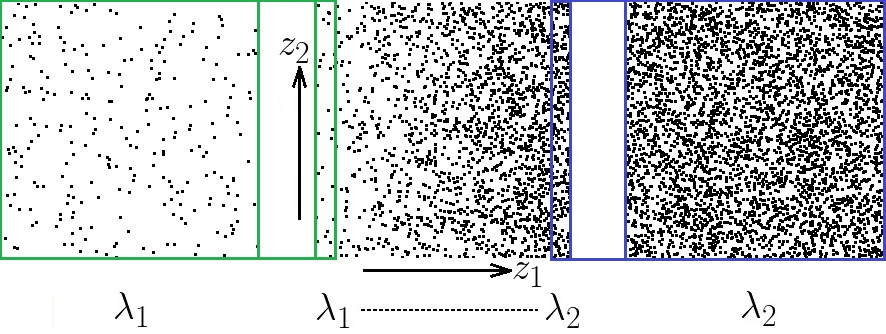
\includegraphics[width=\linewidth]{1-introduction/trend-example}}
			\caption{Пример изображения с трендом, фиксируемого двумя изображениями}
			\label{1-trend-example}
		\end{figure}
	\end{frame}
	
	\begin{frame}{Введение}
		Математически задача синтеза текстуры с трендом описывается с помощью вероятностной постановки задачи обучения:
		\begin{itemize}
			\item Рассматривается многомерное пространство $X$, содержащее множество всех изображений $x$: $X = \{x\}$
			\item Есть обучающая выборка, состоящая из текстур с трендами $D = \{x_i\}$
			\item Считается, что  $D$ задает в $X$ вероятностное распределение $P_X : X \longrightarrow [0,1]$
		\end{itemize}
	\end{frame}
	
	\begin{frame}{Введение}
		Таким образом задача синтеза текстуры из нужного множества сводится к синтезу случайного изображения $x'$ из распределения, близкого к задаваемому обучающей выборкой:
		$$ P_{X'} \approx P_X, \quad x' \sim X'$$
	\end{frame}
	
	\begin{frame}{GAN}
		Генеративные состязательные сети были придуманы в 2014 году и достигли больших успехов в задачах синтеза объектов из сложных распределений.
		\begin{itemize}
			\item Переформулируем: $ P_{X'} \approx P_X \Leftrightarrow \rho(P_{X'}, P_X) \longrightarrow \underset{P_{X'}}{\min} $
			\item $ X' = g_{\theta}(\cdot) \Rightarrow \rho(g_{\theta}(\cdot), P_X) \longrightarrow \underset{\theta}{\min}$
			\item В качестве $\rho$ можно использовать функцию потерь обученного классификатора
		\end{itemize}
	\end{frame}
	
	\begin{frame}{GAN}
		Вводятся две нейросети:
		\begin{itemize}
			\item $d_{\zeta}(x)$ - классификатор для измерения расстояния, \textbf{дискриминатор}
			\item $g_{\theta}(x)$ - сеть, трансформирующая шум в элементы множества $X'$, \textbf{генератор}
		\end{itemize}
		Суть использования двух сетей состоит в том, что они обучаются совместно, конкурируя друг с другом.
	\end{frame}
	
	\begin{frame}{GAN}
		Процесс обучения сети типа GAN принимает следующий вид:
		\begin{columns}
			\column{0.5\linewidth}
			\begin{itemize}
				\item Обучаем дискриминатор при фиксированном генераторе
				\item Обучаем генератор при фиксированном дискриминаторе
				\item Повторяем до сходимости параметров обеих моделей
			\end{itemize}
			\column{0.5\linewidth}
			\begin{figure}
				\centering{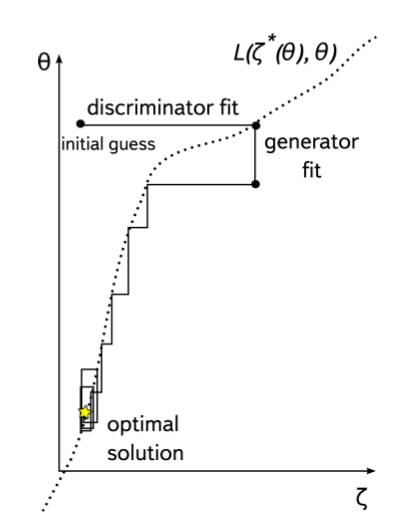
\includegraphics[width=0.75\linewidth]{5-GAN/gan-training}}
			\end{figure}
		\end{columns}
	\end{frame}
	
	\begin{frame}{Оценка качества синтеза текстур}
		Вводится специальная метрика, которая будет учитывать наличие в изображении тренда интенсивности частиц. Рассмотрим среднюю плотность черных пикселей в некотором окне $\xi_k$, и пройдем этим окном по изображению.
		$$\xi_k = \frac{1}{H w}{\sum_{i=k}^{k+w} \sum_{j=0}^{H}\left| \frac{x(i, j) - 255}{255} \right|}, $$$$k = \overline{1, W - w} $$
	\end{frame}
	
	\begin{frame}{Оценка качества синтеза текстур}
		Построив график $\xi(k)$, можно увидеть, как меняется плотность черных пикселей и прослеживается ли тренд.
		
		\begin{figure}[h!]
			\centering{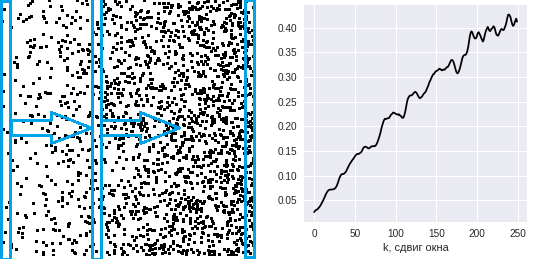
\includegraphics[width=0.75\linewidth]{7-verification/window}}
			\caption{Прохождение окном, W, H - размеры изображения, w - ширина окна.}
			\label{7-window}
		\end{figure}
	\end{frame}
	
	\begin{frame}{Оценка качества синтеза текстур}
		В качестве метрики можно взять среднеквадратичную ошибку:
		$$ \xi = \frac{K}{W-w}\sum_{k=1}^{W-w} (\xi_k - \xi_{0k})^2,$$
		где $\xi_{0k}$ - это $\xi_k$, усредненное по изображениям, содержащим истинный тренд, а $K$ - нормировочный множитель, вводимый для того, чтобы метрики сетей, обученных на разных выборках можно было сравнивать между собой.
	\end{frame}
	
	\begin{frame}{Результаты}
		\begin{table}
			\begin{center}
				\begin{tabular}{p{1.2cm} p{1.2cm} p{1.2cm} p{1.2cm} p{1.2cm} p{1.2cm} p{1.2cm}}
					\toprule
					Вход 1 & Вход 2 & Тренд & nf8 & nf16 & nf16woU & nf32 \\
					\cmidrule(r){1-1}\cmidrule(lr){2-2}\cmidrule(lr){3-3}\cmidrule(lr){4-4}\cmidrule(lr){5-5}\cmidrule(lr){6-6}\cmidrule(l){7-7}
					
\includegraphics[width=1\linewidth]{8-results/sand-trend2/left1}
					&
					
\includegraphics[width=1\linewidth]{8-results/sand-trend2/right1}
					&
					
\includegraphics[width=1\linewidth]{8-results/sand-trend2/pan1}
					&
					
\includegraphics[width=1\linewidth]{8-results/sand-trend2/nf8/gen1}
					&
					
\includegraphics[width=1\linewidth]{8-results/sand-trend2/nf16/gen1}
					&
					
\includegraphics[width=1\linewidth]{8-results/sand-trend2/nf16_woUnet/gen1}
					&
					
\includegraphics[width=1\linewidth]{8-results/sand-trend2/nf32/gen1}
					\\
					
\includegraphics[width=1\linewidth]{8-results/sand-trend2/left2}
					&
					
\includegraphics[width=1\linewidth]{8-results/sand-trend2/right2}
					&
					
\includegraphics[width=1\linewidth]{8-results/sand-trend2/pan2}
					&
					
\includegraphics[width=1\linewidth]{8-results/sand-trend2/nf8/gen2}
					&
					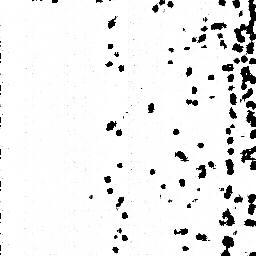
\includegraphics[width=1\linewidth]{8-results/sand-trend2/nf16/gen2}
					&
					
\includegraphics[width=1\linewidth]{8-results/sand-trend2/nf16_woUnet/gen2}
					&
					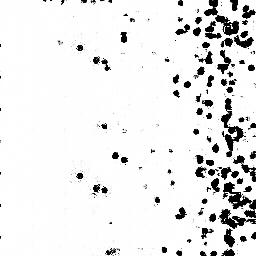
\includegraphics[width=1\linewidth]{8-results/sand-trend2/nf32/gen2}
					\\
					
\includegraphics[width=1\linewidth]{8-results/sand-trend2/left3}
					&
					
\includegraphics[width=1\linewidth]{8-results/sand-trend2/right3}
					&
					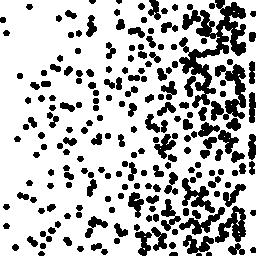
\includegraphics[width=1\linewidth]{8-results/sand-trend2/pan3}
					&
					
\includegraphics[width=1\linewidth]{8-results/sand-trend2/nf8/gen3}
					&
					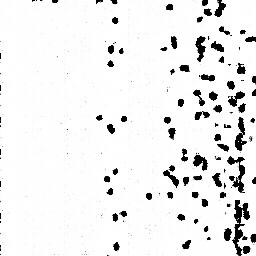
\includegraphics[width=1\linewidth]{8-results/sand-trend2/nf16/gen3}
					&
					
\includegraphics[width=1\linewidth]{8-results/sand-trend2/nf16_woUnet/gen3}
					&
					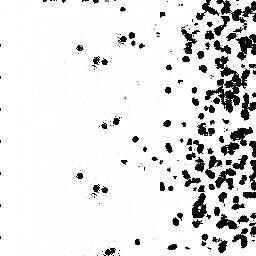
\includegraphics[width=1\linewidth]{8-results/sand-trend2/nf32/gen3}
					\\
					\hline
				\end{tabular}
				\caption{Примеры синтеза (Выборка 1)}
			\end{center}
		\end{table}
	\end{frame}
	
	\begin{frame}{Результаты}
		\begin{figure}
			\centering{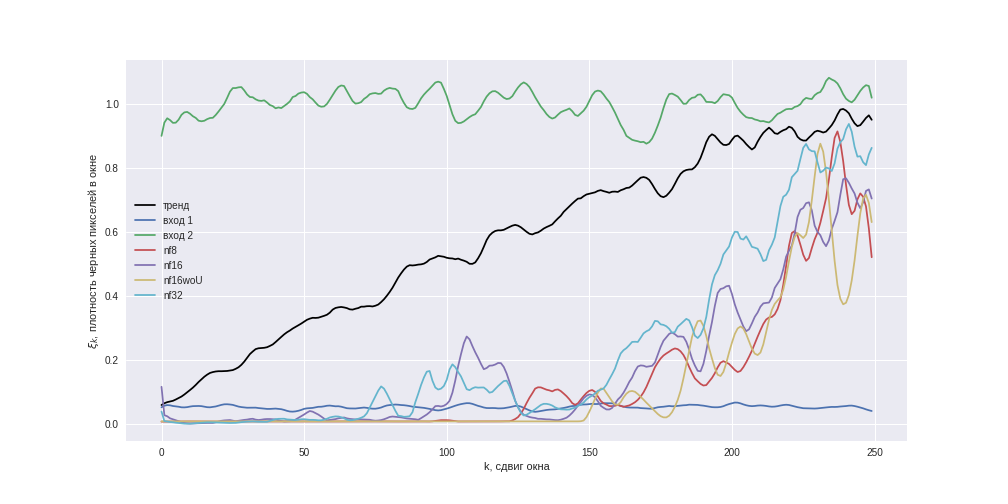
\includegraphics[width=\linewidth]{8-results/sand-trend2/results}}
			\caption{Аппроксимация тренда различными сетями (Выборка 1)}
		\end{figure}
	\end{frame}
	
	\begin{frame}{Результаты}
		\begin{table}[h!]
			\begin{center}
				\begin{tabular}{|c|c|c|c|}
					\hline
					Сеть & Число фильтров на 1-ом слое & Метрика \\
					\hline
					nf16woU & 16 & 0.24048\\
					\hline
					nf8 & 8 & 0.22511\\
					\hline
					nf16 & 16 & 0.18844\\
					\hline
					nf32 & 32 & 0.14589\\
					\hline
				\end{tabular}
				\caption{Значения метрики для разных сетей (меньше - лучше)}
				\label{8-sand-trend2-metrics}
			\end{center}
		\end{table}
	\end{frame}
	
	\begin{frame}{Результаты}
		\begin{table}
			\begin{center}
				\begin{tabular}{p{1.2cm} p{1.2cm} p{1.2cm} p{1.2cm} p{1.2cm} p{1.2cm} p{1.2cm}}
					\toprule
					Вход 1 & Вход 2 & Тренд & nf32e5 & nf64e1 & nf64e5 & nf64e10 \\
					\cmidrule(r){1-1}\cmidrule(lr){2-2}\cmidrule(lr){3-3}\cmidrule(lr){4-4}\cmidrule(lr){5-5}\cmidrule(lr){6-6}\cmidrule(l){7-7}
					
\includegraphics[width=1\linewidth]{8-results/sand-trend8/left1}
					&
					
\includegraphics[width=1\linewidth]{8-results/sand-trend8/right1}
					&
					
\includegraphics[width=1\linewidth]{8-results/sand-trend8/pan1}
					&
					
\includegraphics[width=1\linewidth]{8-results/sand-trend8/nf32e5/gen1}
					&
					
\includegraphics[width=1\linewidth]{8-results/sand-trend8/nf64e1/gen1}
					&
					
\includegraphics[width=1\linewidth]{8-results/sand-trend8/nf64e5/gen1}
					&
					
\includegraphics[width=1\linewidth]{8-results/sand-trend8/nf64e10/gen1}
					\\
					
\includegraphics[width=1\linewidth]{8-results/sand-trend8/left2}
					&
					
\includegraphics[width=1\linewidth]{8-results/sand-trend8/right2}
					&
					
\includegraphics[width=1\linewidth]{8-results/sand-trend8/pan2}
					&
					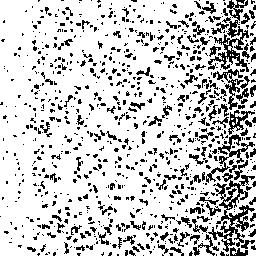
\includegraphics[width=1\linewidth]{8-results/sand-trend8/nf32e5/gen2}
					&
					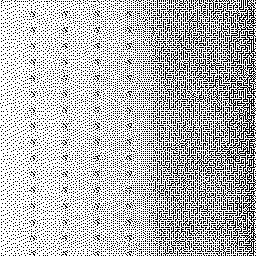
\includegraphics[width=1\linewidth]{8-results/sand-trend8/nf64e1/gen2}
					&
					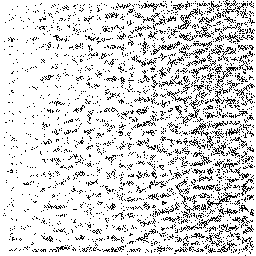
\includegraphics[width=1\linewidth]{8-results/sand-trend8/nf64e5/gen2}
					&
					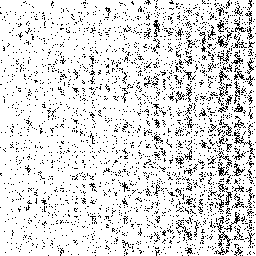
\includegraphics[width=1\linewidth]{8-results/sand-trend8/nf64e10/gen2}
					\\
					
\includegraphics[width=1\linewidth]{8-results/sand-trend8/left3}
					&
					
\includegraphics[width=1\linewidth]{8-results/sand-trend8/right3}
					&
					
\includegraphics[width=1\linewidth]{8-results/sand-trend8/pan3}
					&
					
\includegraphics[width=1\linewidth]{8-results/sand-trend8/nf32e5/gen3}
					&
					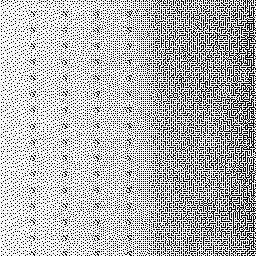
\includegraphics[width=1\linewidth]{8-results/sand-trend8/nf64e1/gen3}
					&
					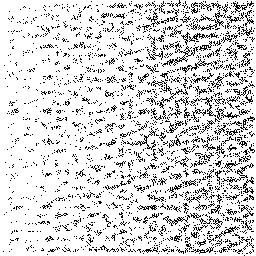
\includegraphics[width=1\linewidth]{8-results/sand-trend8/nf64e5/gen3}
					&
					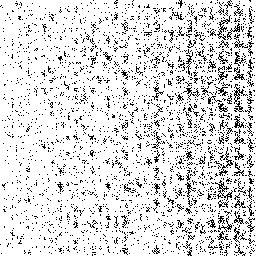
\includegraphics[width=1\linewidth]{8-results/sand-trend8/nf64e10/gen3}
					\\
					\hline
				\end{tabular}
				\caption{Примеры синтеза (Выборка 2)}
			\end{center}
		\end{table}
	\end{frame}
	
	\begin{frame}{Результаты}
			\begin{figure}
				\centering{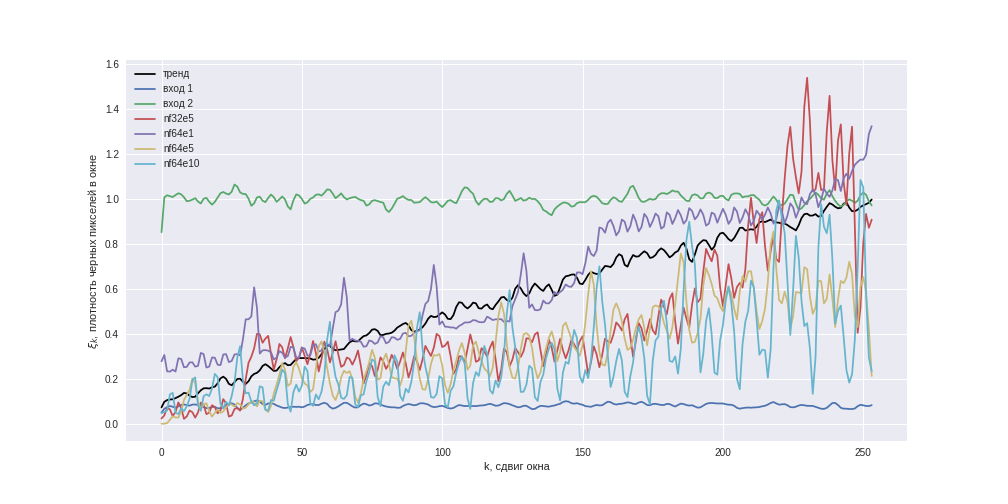
\includegraphics[width=\linewidth]{8-results/sand-trend8/results}}
				\caption{Аппроксимация тренда различными сетями (Выборка 2)}
			\end{figure}
	\end{frame}
	
	\begin{frame}{Результаты}
		\begin{table}
			\begin{center}
				\begin{tabular}{|c|c|c|}
					\hline
					Сеть & Число фильтров на 1-ом слое & Метрика \\
					\hline
					nf64e10 & 64& 0.11168\\
					\hline
					nf64e5 & 64 & 0.06501\\
					\hline
					nf32e5 & 32 & 0.04827\\
					\hline
					nf64e1 & 64 & 0.01393\\
					\hline
				\end{tabular}
				\caption{Значения метрики для разных сетей (меньше - лучше)}
			\end{center}
		\end{table}
	\end{frame}
	
	\begin{frame}{Выводы}
		\begin{itemize}
			\item Исследовано применение архитектуры GAN для синтеза текстур с трендами
			\item Получены результаты синтеза при нескольких наборах гиперпараметров сети на нескольких выборках
			\item Проведено измерение качества генерации для каждого из наборов, используя введенную метрику
		\end{itemize}
		Результаты показывают на возможность применения GAN для синтеза текстур с трендами.
	\end{frame}
	
	\begin{frame}
		\centering\huge{Спасибо за внимание!}
	\end{frame}
	
	\begin{frame}{Минимизационная задача}
		Обучение нейронной сети является задачей многопараметрической оптимизации функционала потерь. Для используемых в этой работе сетей данная задача ставится так:
		 $$ L(G, D) = L_{adv}(G, D) + \eta L1$$
		 $$L1 = \mathbb{E}_{p_{data}(s_1, s_2, r)} (\parallel r - G(s_1, s_2) \parallel_1)$$
		 $$ L_{adv}(G, D) = \mathbb{E}_{p_{data}(s_1, s_2, r)}\log D(s_1, s_2, r)+ $$
		 $$ +  \mathbb{E}_{p_{data}(s_1, s_2)} \log (1 - D(s_1, s_2, G(s_1, s_2))) $$
		 $$ D^* = \underset{D}{\arg\min} L(G^*, D)  $$
		 $$ G^* = \underset{G}{\arg\min} L(G, D^*)  $$
	\end{frame}

\end{document}